% begin module implicit-differentiation-ex1
\begin{frame}
\begin{example}[Example 1, p. 165]
\begin{columns}[t]
\column{.5\textwidth}
\abovedisplayskip=0pt
\belowdisplayskip=-15pt
\abovedisplayshortskip=0pt
\belowdisplayshortskip=0pt
\begin{align*}
\text{If } x^2+y^2 & = 25, \text{ find }\frac{\diff y}{\diff x}.\\
\uncover<2->{%
\alert<handout:0| 3>{\frac{\diff}{\diff x} (x^2+y^2)}%
}%
& \uncover<2->{ = } %
\uncover<2->{%
\alert<handout:0| 4-5>{\frac{\diff}{\diff x} (25)}%
}\\%
\uncover<3->{%
\alert<handout:0| 3>{%
\alert<handout:0| 6-7>{\frac{\diff}{\diff x} (x^2)}%
 + %
\alert<handout:0| 8-9>{\frac{\diff}{\diff x} (y^2)}%
}}%
& \uncover<3->{ = } %
\uncover<5->{%
\alert<handout:0| 5>{0}%
}\\%
\uncover<6->{%
\alert<handout:0| 6-7>{\uncover<7->{2x}}%
 + %
\alert<handout:0| 8-9>{\uncover<9->{2y\frac{\diff y}{\diff x}}}%
}%
& \uncover<6->{ = } %
\uncover<6->{%
0%
}\\%
\uncover<10->{%
2y\frac{\diff y}{\diff x}%
}%
& \uncover<10->{ = } %
\uncover<10->{%
-2x%
}\\%
\uncover<11->{%
\frac{\diff y}{\diff x}%
}%
& \uncover<11->{ = } %
\uncover<11->{%
-\frac{x}{y}%
}\\%
\end{align*}
\column{.5\textwidth}
Find an equation of the tangent line to the circle $x^2 + y^2 = 25$ at $(3,4)$.

\uncover<12->{Plug in $x = 3$, $y = 4$:}
\abovedisplayskip=0pt
\belowdisplayskip=0pt
\[
\uncover<12->{%
\frac{\diff y}{\diff x} = -\frac{3}{4}
}%
\]
\uncover<13->{%
Point-slope form:
\abovedisplayskip=0pt
\belowdisplayskip=0pt
\[
y - 4 = -\frac{3}{4}(x - 3)%
\]
}%
\begin{center}
\ \only<handout:0| -12>{%
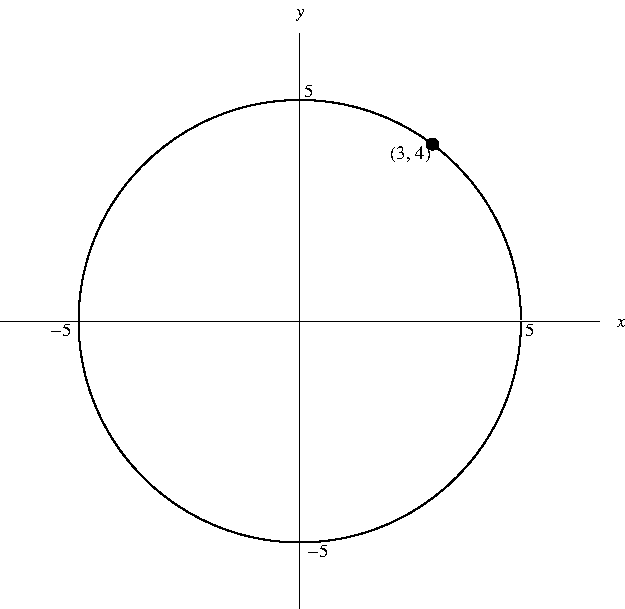
\includegraphics[height=3.5cm]{implicit-differentiation/pictures/03-06-ex1a.pdf}%
}%
\only<13->{%
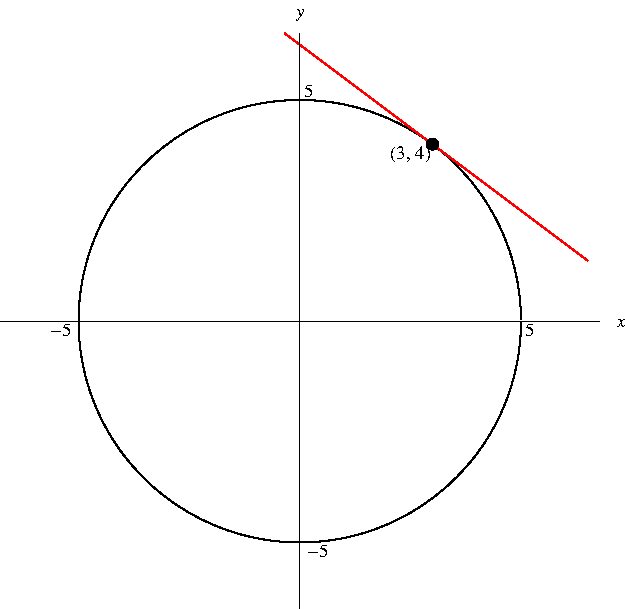
\includegraphics[height=3.5cm]{implicit-differentiation/pictures/03-06-ex1b.pdf}%
}%
\end{center}
\end{columns}
\end{example}
\end{frame}
% end module implicit-differentiation-ex1
